\documentclass{standalone}
\usepackage{tikz}
\usepackage{pgfplots}
\pgfplotsset{compat=1.12,width=5cm}%
\begin{document}
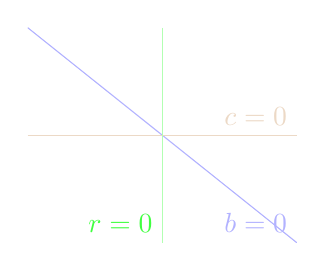
\begin{tikzpicture}
\newcommand{\mx}{.15}
\begin{axis}[hide axis,xmin=-\mx,xmax=\mx,ymin=-\mx,ymax=\mx,width=5cm]
\newcommand{\fclr}{blue!30}
\draw[\fclr] 
	(-\mx,\mx) 
-- (\mx,-\mx) node[above left]{\(b=0\)};
\newcommand{\gclr}{brown!30}
\draw[\gclr] (-\mx,0) -- (\mx,0) node[above left] {\(c=0\)};
\draw[green!30] (0,\mx) -- (0,-\mx);
\node[above left,green!75] at (0,-\mx) {\(r=0\)};
\end{axis}
\end{tikzpicture}
\end{document}
